\section{
%Constructing 
%natural 
%the concept hierarchy and relationships
Roles, competency questions and conceptual model}

\label{section:3}

As mentioned, our starting point for examining the required coverage for scholarly knowledge graphs were the researcher needs associated with their research-related activities.
Our approach is thus more `human-centric', compared to `data-centric' approaches to scholarly KG requirement analysis, which primarily look at what is already available in structured databases and KGs.

We started with identifying the \emph{roles} fulfilled by researchers and entailing information foraging from external sources. 
For this purpose, the two senior co-authors (VS and OC) went through their comprehensive CVs and/or daily activity log, and distilled from the activities and achievements a set of distinct roles. 
%Our model is based solely on competency questions. Hence our approach is to start by identifying types of stakeholders interested in the construction and/or use of the knowledge graph.  %Researchers can play different roles in different contexts throughout their career repeatedly, hence w
The following roles (partially grouped, for brevity) have been identified:

\begin{itemize}
    \item Researcher (general) - researching and publishing
    \item Leader of a research group  (or of a more formal unit such as a Department)
    \item Advisor (of PhD students, or generally, more junior colleagues)
    \item Event organizer / Volume editor / Journal board member
    \item Evaluator of publications, researchers, organizations/groups, projects, and funding programs
    \item Research project proposer / manager
    \item Industry transfer mediator / recruiter.
\end{itemize}

%At first, we also included entities of the more academic/educational context such as \textit{teacher}, \textit{student}, and of the more industrial and public context such as \textit{journalist}, because there exist competency questions involving them. In the end, we have decided to limit our scope to focus mainly on the domain of research due to extensive and unnecessary complexity. However, it is still a considerable possibility to include these concepts and extend our model to achieve a broader and more comprehensive ecosystem.

%After having identified the significant roles of a researcher, our next step is to identify what kinds of applications could make use of public scholarly knowledge graphs with the underlying ontologies based on our model. This is to create a holistic presumption of which competency questions should arise. The knowledge base could contain basic data about individual researchers and their work, which is trivial and could be solved in many conventional ways. Such applications include generation of researcher CVs, summarized dashboards of academic organizations or research groups, basic search for researchers and research projects. However, the advantages of modeling a model of thoroughly interconnected concepts using ontologies is the ability to exploit the linkage and relationships between many data instances as well as making use of reasoners to derive facts. This opens up and leverages a wide range of potential use cases for applications which can provide richer, more relevant and extensive experiences for users in many context. Such applications include faceted research lookup, smart research recommender, research topic aggregator \& statistical analysis, research data miner, researcher timelines, research contributions referencer.

For each researcher role, we formulated several verbal \emph{competency questions} (CQs) and equipped them with \emph{paths} of high-level concepts and relationships whose instantiations should  provide answers to the questions in a hypothetical KG. An example of path is \texttt{RESEARCHER - ORGANIZATION - EVENT}. This way, we created a set of paths from which we then constructed a holistic, highly abstract \emph{conceptual model} presented in Figure \ref{relationship-model}. We also gathered the terms in these paths into a separate collection. These terms were later put into a logical hierarchy, as shown in Figure \ref{natural-concept-hierarchy}. To reduce the complexity of the conceptual model, we only show ten top-level terms in it.
In Table \ref{tab:competency-questions} we showcase several chosen CQs and associated paths.
(To demonstrate the wider scope of the conceptual model, we omit the roles of `general' researcher and publication writer, as these have been the main focus of most previous initiatives surveying  scholarly ontologies/KGs.
They are however also part of our complete CQ set.)%, which is available on our research repository\footnote{\url{https://github.com/nvbach91/iga-knerd}})

\begin{table}[]
\caption{Examples of high-level competency questions and entity type paths}
\label{tab:competency-questions}
\begin{tabular}{|p{6cm}|p{6cm}|}
\hline
%\multicolumn{2}{|l|}{\textbf{Researcher CQ}}                                                                                                                                                                                                                                                           \\ \hline
%What has been researched / written on this topic?                                                                                                     & Topic - Project - Publication                                                                                                                  \\ \hline
%Who already had projects on this or similar topic?                                                                                                    & Researcher - Project - Topic - Topic                                                                                                           \\ \hline
%Who cites my publications?                                                                                                                            & Researcher - Publication - Publication                                                                                                         \\ \hline
\multicolumn{2}{|l|}{\textbf{Research Group Leader / Advisor CQ}}                                                                                                                                                                                                                                      \\ \hline
What positions (in projects, or general) in other organizations may attract junior researchers as an alternative to working in my group?                                            & $\bullet$ Topic - Project - Organization \newline $\bullet$ Topic - Position - Organization                                                                                                                     \\ \hline
\multicolumn{2}{|l|}{\textbf{Research Event Organizer / Volume Editor / Journal Board Member CQ}}                                                                                                                                                                                                      \\ \hline
Who should I invite as keynote speaker or reviewer (based on thematic relevance, research quality, and history of engagement in this or similar events)?       & $\bullet$ Topic - Publication - Researcher - \newline Assessment \newline $\bullet$ Topic - Researcher - Assessment \newline $\bullet$ Publication Venue - Publication - \newline Researcher - Assessment       \\ \hline
\multicolumn{2}{|l|}{\textbf{Evaluator of publications CQ}}                                                                                                                                                                                                                                            \\ \hline
What has been researched / written on the topic this publication deals with?                                       & $\bullet$ Publication - Topic - Publication \newline $\bullet$ Publication - Topic - Project                                                                               \\ \hline
What has the author previously published on this topic? What is the overlap with the current paper?                                                   & $\bullet$ Publication - Researcher - Publication - Topic                                                                                                 \\ \hline
How does the paper comply with the standard criteria of scientific writing?  
What argument is used by an author or a reviewer in a publication/review? & $\bullet$ Publication - Assessment\newline
$\bullet$ Publication - Review - Argument

\\ \hline
\multicolumn{2}{|l|}{\textbf{Evaluator of researchers CQ}}                                                                        \\ \hline
How important are the venues where the researcher publishes?                                                                                         & $\bullet$ Researcher - Publication Venue - \newline Assessment                                                                                                    \\ \hline
How much technology transfer activity (to industry) does a researcher do?                                                                             & $\bullet$ Researcher - Organization                                                                                                                      \\ \hline
%\textbf{Evaluator of academic institutions / groups}                                                                                                  &                                                                                                                                                \\ \hline
%How many publications, and of what kinds, has the institution published?                                                                              & Organization - Researcher - Publication                                                                                                        \\ \hline
%How much scientific outreach is done by researchers in the institution? (E.g., events and publications for the general public)                        & Organization - Event \newline Organization - Researcher - Publication                                                                                  \\ \hline
\multicolumn{2}{|l|}{\textbf{Evaluator of projects CQ}}                                                                \\ \hline
How topical are the goals of the project, in terms of problems addressed? Do people often write on these problems? Are they encouraged by funding programs?          &  $\bullet$ Project - Goal/Problem - Publication - \newline Researcher\newline                     $\bullet$ Project - Goal/Problem - Program                                        \\ \hline
\multicolumn{2}{|l|}{\textbf{Project proposer CQ}}          \\ \hline
                              What are the preferred topics of the program/call? What are the topical problems in the field? &
$\bullet$ Program - Topic - Problem
                      \\ \hline
Who has experience with previous projects in the chosen program?
&
$\bullet$ Program - Project - Researcher 
                      \\ \hline
What partners should be invited for such a kind of project, based on the problem addressed?
&
$\bullet$ Problem - Publication - Researcher - \newline Organization\newline
$\bullet$ Problem - Method - Researcher - Organization
                      \\ \hline
What is the usual budget of projects in this program?
&
$\bullet$ Program - Project
                         \\ \hline
%\multicolumn{2}{|l|}{\textbf{Evaluator of programs CQ}}                                                                                                                                                                                                                                                \\ \hline
%How successful are the projects funded by this program?                                                                                               & Funding Program - Project - Publication - Publication Venue - Assessment; Funding Program - Project - Method/Patent; Funding Program - Project \\ \hline
%\multicolumn{2}{|l|}{\textbf{Project proposer CQ}}                                                                                                                                                                                                                                                     \\ \hline
%What are the preferred topics of the program/call? What are topical problems in the field?                                                            & Funding Program - Topic                                                                                                                        \\ \hline
%Who has experience with previous projects in the chosen program?                                                                                      & Funding Program - Project - Researcher                                                                                                         \\ \hline
\multicolumn{2}{|l|}{\textbf{Industry transfer promotor CQ}}                                                                                                                                                                                                                                           \\ \hline
Which company or other organization is active in the given field, as a potential transfer target?                                                     & $\bullet$ Project - Topic - Organization                                                                                                                 \\ \hline

\end{tabular}
\end{table}

%We then proceeded to composing a list of glossary terms of research-relevant concepts and constructing their natural hierarchy based on interviewing and examining activity journals of two senior researchers who have gone through most of their research and pedagogic career. 
The hierarchy in Figure \ref{natural-concept-hierarchy} shows six of the top-level concepts, further broken down to subtypes. The scope and purpose of each concept are as follows:
\begin{itemize}
    \item The \textit{Topic} concept may refer to research areas, research problems, methods etc.; namely, to anything that can be referred to as the subject of publications, of activities by research projects, research groups, funding programs, events, etc. Even `tangible' assets used for research, including software and datasets, may be considered as a research topic in this context.

    \item The \textit{Event} concept refers to scientific events such as conferences or seminars, and relates, e.g, to the on what kind of events can an organization organize or and which researchers have been involved in it through their publications.
% can a researcher be involved in an event without a publication?

    \item The \textit{Assessment} concept refers to various evaluations of the quality of organizations, researchers, research projects, research publications (i.e. peer- or professional reviewing) and publication venues. The quality can be represented by metrics, rankings, certifications, textual reviews, etc.

    \item The \textit{Organization} concept is a parent concept to the types of organizations or working units that a researcher might be engaged in; some types of organizations can also offer funding programs and support the research projects of researchers, or be the recipients of the academic know-how. We  identified 6 subtypes as follows: \textit{NGO}, \textit{Foundation}, \textit{Academic Institution}, \textit{Research Group}, \textit{Company}, \textit{Government Body}. The important concept of \textit{Research Spin-off} is a special type of \textit{Company}. 

    \item The \textit{Publication} concept has 5 subtypes, which distinguish between different publication purposes and publishing formats. For example, an \textit{Edited Collection} can be a book, proceedings, a journal special issue, or any other thematically coherent collection of individual publications, typically with a preface or editorial (its writing is a part of authoring this kind of publication). An \textit{Outreach Publication}'s purpose is to connect science with the society. It can be a magazine article, a press release, etc.

    \item The \textit{Publication Venue} concept refers to different parts of types of publication venues can researchers submit their manuscripts to.
\end{itemize}

\begin{figure}
\centering
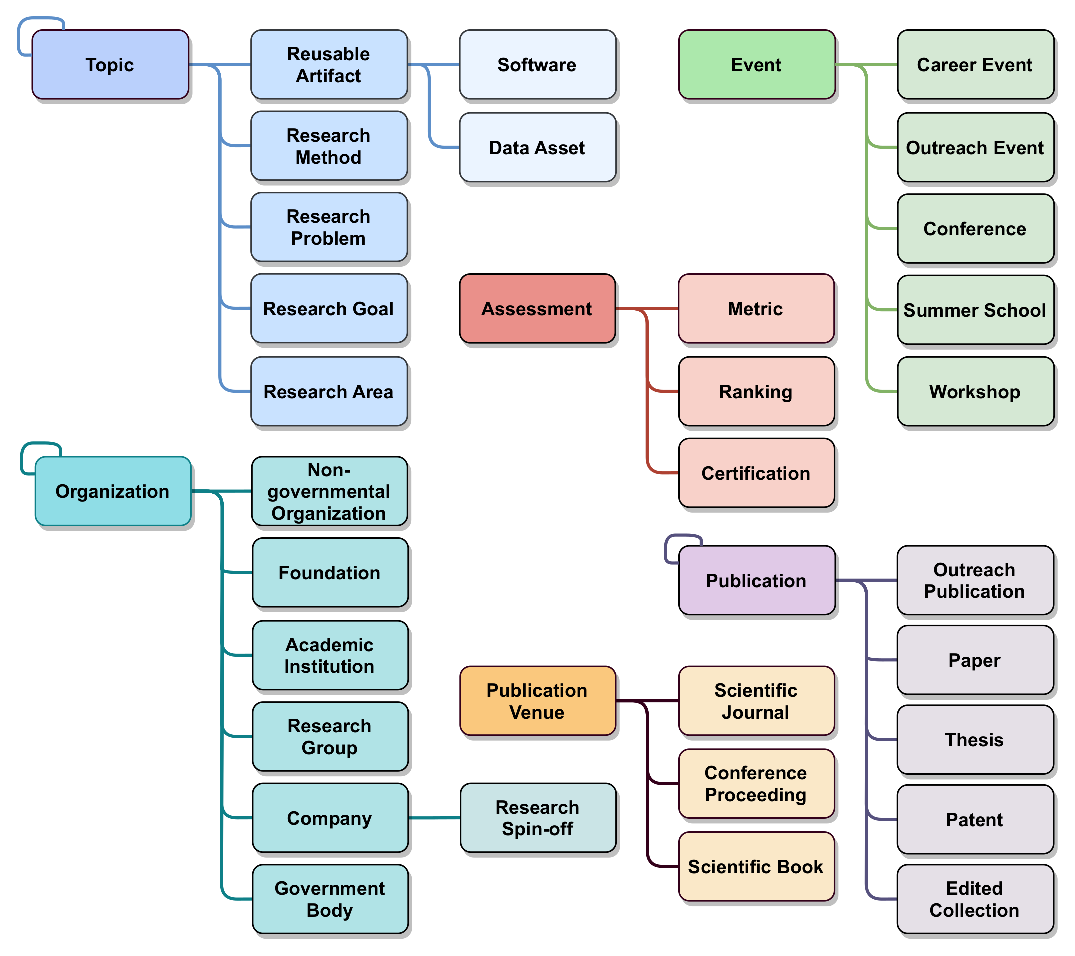
\includegraphics[width=8cm]{figures/natural-concept-hierarchy.eps}
\caption{Natural concept hierarchy} \label{natural-concept-hierarchy}
\end{figure}


All mentioned relationships in the previous descriptions of top-level concepts are captured in Figure \ref{relationship-model}. In this model, there are 3 other top-level concepts that do not have a further breakdown. We describe them as follows:


\begin{itemize}
    \item A \textit{Researcher} %top-level concept is the main actor. Researchers 
    can, e.g., be a member of organizations and can contribute to research projects and publications. %Through the \textit{Research Contribution} concept, t
    The researcher also has access to other concepts such as \textit{Event} and \textit{Publication Venue}.
    
    \item The \textit{Position} concept is used to describe possible positions or roles of a researcher within an organization.% and determine what kind of contribution does the researcher has within a project or a publication. % what about events?
    
    \item The \textit{Funding Program} concept models a source of funding for research projects, possibly assigned across multiple calls.

    \item A \textit{Project}  %refers to an organized and planned work of researchers.
    may be proposed and solved by researchers (in some positions) or organizations,  supported by funding programs, and associated with publications.% since they are one of their main outputs. The relationship with the term Position serves as the specific role of a researcher in the project.
    
    %\item The \textit{Publication Citation} top-level concept is used to describe which publication is cited by other publication and the overall relationship between publications and projects. %can a research project be cited without a publication?
    
    %\item The \textit{Publication Review} top-level concept is used to describe the role reviewer of a researcher in the reviewing process of a paper. %although this is not public info?
\end{itemize}

Note that the paths are not disambiguated, and in many cases may correspond to semantically different kinds of relationships, e.g., Researchers may provide assessments on something, but can also be assessed by other researchers.

\begin{figure}
\centering
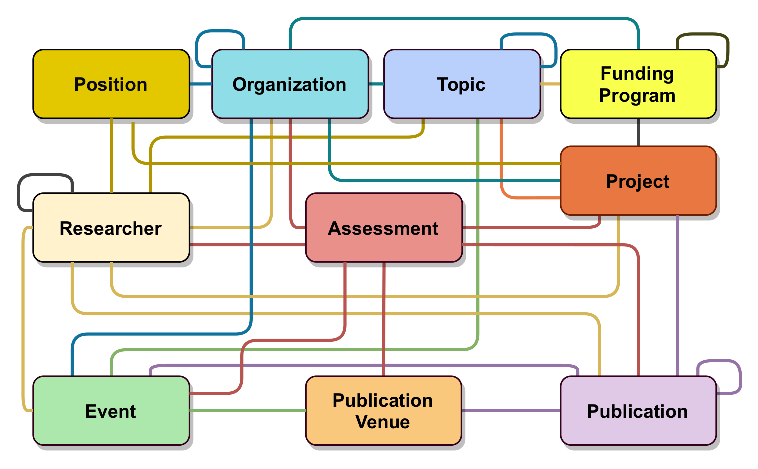
\includegraphics[width=7cm]{figures/relationship-model.eps}
\caption{High-level relationship model} \label{relationship-model}
\end{figure}
